\newpage
\section{Subjects and Shared Input Pools}

Shared input pools have the same structure like subject-specific ones, and thus, the same properties like the standard input pool. The only difference is that different subjects can deposit in or remove messages from a shared input pool. Subjects that want to send a message via a shared input pool do not use a subject name as addressee of a message, but the name of a shared input pool instead. In a distributed system several shared input pools for different purposes can be used. Figure 7 shows the slightly changed structure of the traffic management system when operating it with a shared input pool \todo{CS: hier fehlt das originäre Beispiel als Bezugspunkt.} The subject "Car detection" represents the shared input pool.


\begin{figure}[htbp]
	\centering
	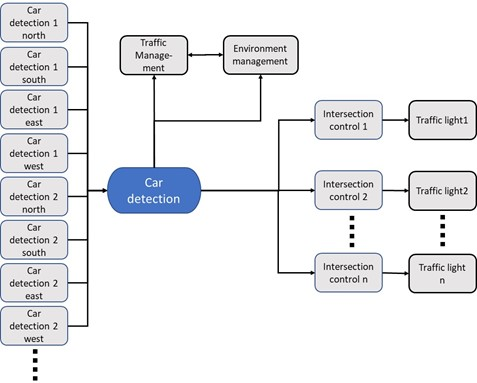
\includegraphics[width=0.9\linewidth]{Figures/Chapter5/figuresshared/SharedInputPoolExample.jpg}
	\caption[Traffic Management System with Shared Input Pool]{Traffic Management System with Shared Input Pool}
	\label{fig:SharedInputPooTraffic}
\end{figure}


Shared input pools make a distributed system more flexible when additional participants or nodes are added. For instance, a third intersection control could be added to the traffic management system without much effort. In this case, only the additional detectors and the components for controlling the intersection have to be complemented and linked to the shared input pool. The extension would have no impact on the behavior of the other subjects and their behavior in that system.
There is one additional attribute for shared input pool: It defines whether a message will be removed from the input pool once a message has been picked up by a receiving subject. This mechanism is required, since several subject may need to process a particular message. In addition, it allows keeping historical information in the input pool, in particular for analyzing the content of an input pool independently of the behavior of interacting subjects.
The messages of an input pool can be analyzed with respect to certain patterns of its messages. In order to perform such an analysis, Complex Event Processing (CEP) concepts can be applied. Complex Event Processing can be encapsulated in a subject. A subject of this kind scans the messages of a shared input pool and checks whether patterns of interest can be found. Once such a pattern is identified, a message including the discovered pattern can be sent to other participants, and initiate further activities. Figure 8 shows the traffic management example enriched with subjects processing complex events.
In the example, the subject "CEP pollution analyzer" can analyze the time between cars passing the intersection in a certain time period. It can identify the events "low traffic" or "high traffic" and send it to the subject "Environment management". In case of tunnels, the subject "Environment management" might react to this information in a different way compared to open air settings.


\begin{figure}[htbp]
	\centering
	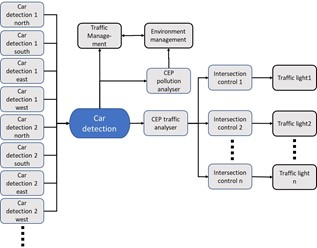
\includegraphics[width=0.9\linewidth]{Figures/Chapter5/figuresshared/SharedInputPoolEvent.jpg}
	\caption[Shared Input Pools and Complex Event Processing]{Shared Input Pools and Complex Event Processing}
	\label{fig:sharedInputPoolEvents}
\end{figure}

\subsection{Implementing Shared Input Pools}
As mentioned earlier, shared data repositories represent a single point of failure of a distributed system. A malfunction of a shared data storage component or device may have a significant impact on the functionality of the whole distributed system. If a subject or a communication line is disturbed, only a small part of a system may be concerned but if a shared data store is down this has an impact on all subjects accessing this input pool.
\\
In addition to this operational problem it must be decided in the course of organizational implementation which organization is held responsible for running and maintaining the system hosting the shared data. Such issues become prominent, if a distributed system is connecting several independent organizations, e.g., different companies in a supply chain. Distributed systems run by independent organizations may also have to deal with several changes dynamically, affecting the data quality and system stability. Even companies can be replaced by other organizations. If only functional subjects are concerned, such a change can be managed without affecting the operation of the entire system: The execution of a subject is just assigned to the new actor. The problem is more serious if a company leaving a distributed system is responsible for running the system with shared data, as other participants of the shared system are affected. Then, a new company still part of the distributed system must take over the responsibility for the shared data. The migration of these data from one company to another can become very cumbersome from the business point of view and from a technological perspective, too.
One way to solve these problems is implementing shared input pools with blockchain technology. A blockchain is an open, distributed ledger that can record transactions efficiently in a verifiable and permanent way. Blockchains allow to achieve the integrity of a collection of data in a distributed peer-to-peer system, whereas the number of the peers is unknown and an unknown number of them are not reliable and trustworthy \cite{book:Blockchainbasics}.
\\
Today, blockchains are mainly used for managing the ownership of money, goods, real estates, etc. Each participant in a distributed system may have a copy of a blockchain. Changes in a blockchain follow a mechanism which manage changes in a consistent way and the change protocol guarantees that any participant will have again a consistent copy after a change. A change of a blockchain means that a new data record is added, and nothing can be removed from a block chain. Adding a new block to a block chain requires some effort from parties involved in a blockchain. This effort is rewarded by adding crypto money to the party when having accomplished the task successfully. These rewards serve as an incentive for the creators of blocks.
\\
Although heavily questioned with respect to effort and gains by practitioners \cite{article:BlockchainUniverse} blockchain technology provides concepts ensuring the trustworthiness of system components. The latter becomes crucial when operating sensitive distributed systems, such as public transportation and healthcare, in particular when event-based data fusion is needed, where nodes of various type (sensor systems, vendor-specific monitoring systems. user devices, household items, etc.) exchange notifications of events and decision-relevant data with each other. In such settings, not only notification mechanisms needs to be streamlined in case of heterogeneity of nodes, but also data source trust is important for further processing and system behavior \cite{article:EventbasedSensor}.
\\
In order to ensure dependable sharing of data, these basic properties of blockchains need to be adapted to the requirements of a shared input pool. Hence, a blockchain-oriented implementation of a shared input pool must meet several requirements:
\begin{enumerate}
	\item Subjects can subscribe for the access to a shared input pool.
	\item Subjects subscribed for an input pool may deposit or read events from that input pool.
	\item Events can be marked as removed from a shared input pool.
	\item Subjects may analyze the content of a blockchain, e.g., when processing complex events.
	\item There must be a mechanism that a block chain can be deleted, once all involved parties agree on that.
\end{enumerate}

Traditionally data received from "things" are not very complex. These data are mainly values as measured by sensors, or binary signals. This may lead to a paradox situation: If such simple data are to be stored in a blockchain, the fee to be paid for adding blocks containing simple data is larger than the value being transferred.
One way to solve the resulting incentive problem is to use permissioned block chains instead of open block chains: Blockchains for dedicated distributed application are not open blockchains like the ones implementing the management of digital currencies.
\\
For the implementation of shared input pools, we suggest managed or permissioned blockchains. For instance, Hyperledger Fabric \cite{article:hyperledger} is an open source implementation of a permissioned blockchain. Unlike to a public permissionless network, the participants are known to each other, rather than staying anonymous and interacting untrusted. It means, while the participants may not fully trust one another, e.g., in case of being competitors in the same industry sector, a network can be operated under a governance model that is built on the extent of trust existing between participants, such as a legal agreement or framework for handling disputes. When building a business process with known participants, such type of a blockchain implementation would be sufficient. Consensus algorithms for permissioned blockchains are faster and do need much less energy than permissionless blockchain networks.
\\
In \cite{article:Blockbench} it is reported that hyperledger fabric is the fastest available permissioned blockchain. The transaction throughput could even be increased from 3,000 to 20,000 transactions per second \cite{article:hyperledgerfabric}.
\\
When using Hyperledger to create blockchain networks of that kind, a hyperledger blockchain network provides a technical infrastructure offering ledger and smart contract (chaincode) services to applications. Primarily, smart contracts are used to generate transactions which are subsequently distributed to each peer node in the network where they are immutably recorded on their copy of the ledger. The users of applications can be users of client applications or blockchain network administrators.
\\
Subject add messages to the shared input pool and other subjects want to read these messages. If a shared input pool is implemented as a blockchain it is necessary that the chain code (smart contract in Ethereum) realizing the functions of the shared input pool must interact with the world outside the block chain. In hyper ledger fabric (including Ethereum), this problem is solved by so called oracles. We suggest using the blockchain patterns Oracle and Reverse Oracle as described in \cite{book:Blockchainapplications}. For flexibility reasons we prefer off chain oracles - see figure \ref{fig:sharedblockchain}.



\begin{figure}[htbp]
	\centering
	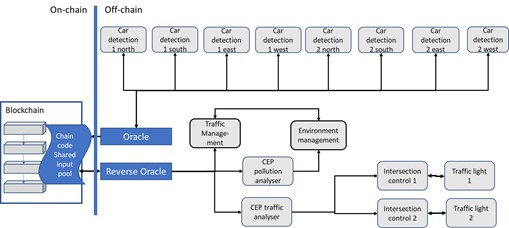
\includegraphics[width=0.9\linewidth]{Figures/Chapter5/figuresshared/Block-Chain.jpg}
	\caption[Utilizing block chain patterns Oracle and Reverse Oracle]{Utilizing block chain patterns Oracle and Reverse Oracle}
	\label{fig:sharedblockchain}
\end{figure}

\subsection {Conclusion}
The more the Internet of Things (IoT) propagates into domain-specific applications, the more stakeholders get involved with respect to business and user requirements. They expect omnipresent use and adaptation on demand. Ensuring robust and semantically correct operation in dynamically networked IoT environments requires tools and development methods to handle complex patterns of interactions due to the different components and capabilities of actors.\\
These patterns refer to the (reactive) flow of control and correct exchange of data. We have proposed an integrated approach based on subject-oriented process models. These role-specific representations allow behavior abstractions on various levels of granularity and can be enriched with a mechanism for handling complex events and sharing data. The data handling mechanism is bound to exchanging messages and a blackboard-like structure. Its behavior can be implemented through blockchain technologies, in case a single point of failure in system operation should be inhibited. The latter is of crucial importance, once the data exchange between IoT-system elements should be trustworthy and traceable.\\
The presented approach should facilitate transparent development and stakeholder understanding of (complex) IoT systems in dynamic settings, due to the implementation-independent representation on a mainly diagrammatic level based on a minimalistic notation, stemming from subject-oriented modeling. Abstractions and decomposition into IoT system components encapsulate behavior. The overall behavior of an IoT system is determined by a set of interactions that integrates the control flow with data exchange patterns from a semantic process perspective. Application design can be understood as top-down approach with the functionality specific to the IoT application residing on an edge operating system. Platform services implement all functional requirements, and are backed by communication and information processing technologies. Cross-functional issues, such as secure operation, business-relevant standardization, and critical event handling can be explicated on an implementation-independent level due to the semantic process representation scheme. The resulting models are executable and thus, can be adapted dynamically.


\subsection{Future Work}

Due to the novel conceptual integration addressed, several aspects and topics need to be addressed by future research:
\begin{list}{-}{spacing}
\item From an application perspective, the results need to be aligned with novel industry 4.0 concepts (cf. [29]), since there not only existing standards are framed by business processes, but also distributed operation of production-relevant processes and real-time sharing of data.
\item From an implementation perspective, our approach requires a (prototypical) realization of an appropriate block chain mechanism for managing shared input pools meeting all requirements in section 4.
\item From an industry perspective, performance evaluations might lead to reconsider our conceptual findings, e.g., how to manage a shared input pool of a distributed system in real time.
\item Definition of structural semantics in OWL
\item Definition of execution semantics in ASM
\end{list}